\chapter{Extended abstract \label{sec:resumenIngles}}

Because of the digital transformation process that is happening nowadays in the society, specially, in the business world, data generation and traffic has grown very abruptly. Every day, millions of Terabytes of new data are generated \cite{BDStats}.

The origin of this data is very varied but the main reason of this exponential growth is the irruption of the connected devices in the daily life of the people. Specifically, the increase in the numbers of the smartphones in use \cite{phoneGrowth} and, more recently, the apparition of the Internet of the Things (IOT) and the wearables, are the main drivers in this growth of the quantity of data generated.

This great volume of data makes the processing task a very costly operation in perspective with the past. Moreover, the use of different sources makes the data structure heterogeneous, increasing the complexity of the processing job. This two issues has made necessary the development of new tools that achieve this task, known as \textit{big data}.

The objective that business and organizations has with the use of this technology is to get valuable information for them that help to structure their market strategy and take some advantage from their competitors. But there are also organizations and public actors that are using these tools to improve the efficiency of some systems. Real time analysis is gaining special relevance nowadays for this optimizing task, for example in traffic systems.

In this Final Degree Project, we are going to take as starting point the challenge gave during the 2015 \gls{DEBS} Grand Challenge. We are going to work with all the traces of the trips made during 2013 by the New York City taxis, which were more than 170 million of trips, and we will do some queries in them, measuring the efficiency of the systems used. There will be two queries, one that search the top ten frequent routes and the top ten profitable areas for the taxi driver, both of them taking in consideration a time window to do it.

In this document we will present the designs of the \textit{big data} architecture implemented. This architecture will be based and developed in \textit{Apache Spark} \cite{spark} in all of its implementations and the distributed file system of \textit{Apache Hadoop} \cite{hadoop} in some. \textit{Apache Parquet} \cite{parquet} will be used for the files to save the processed data as a file type.

To obtain the required results, the user will have to interact with the \textit{big data} system. The first step, after getting the data, will be loading the data. This data will be processed by the system to accommodate the data to the requirements of the challenge. The last step will be the data analysis of the processed data to obtain the results of the queries.

\section{Objetives}
The main objective of this project is the design and implementation of a scalable and efficient \textit{big data} system that address the queries proposed in the \gls{DEBS} Grand Challenge of 2015. To achieve this goal, the project will have the next work phases:

\begin{itemize}
\item Analysis and study of \textit{big data} paradigm and tools available nowadays.

\item Study of the problem to solve, both the data given and the questions to solve.
	
\item Design of the \textit{big data} architecture for the different configurations and situations that are going to be tested.
	
\item Implementation of the different versions of the \textit{big data} architecture designed for the environments that will be tested.
	
\item Design and implementation of the classes and scripts that are going to be responsible of the data processing and the execution of the queries.
	
\item Execution of the scripts developed to make the test and obtain the results both the data and the execution time and system efficiency.
	
\item Analysis of the results, comparing the designs tested in varied environments and configurations.
	
\item Starting off the analysis of the results, conclusions and future lines of work.
\end{itemize}

\section{State of the art}
In this section, the context and the state of the technologies that will be used in this project will be analysed. To do so, we are going to describe the actual situation of open data, \textit{big data} and the tools Apache Spark, Hadoop and Parquet.

\subsection{Open Data} 
In this project, we are going to use the traces of all the trips done in 2013 by all the yellow cabs of New York city. This data is available because of a \Gls{FOIL} petition that Chris Whong made. Nowadays, this tendency is changing and more data is being uploaded for free by organizations and governmental organisms.

This kind of data is called open data, it is information that is available for everyone without any kind of limitations like copyright, patents or other type of control mechanism. This data could be used and distributed with total freedom by anyone \cite{opendata}.

This movement that is being held for a great number of governmental and no-governmental organisms \cite{onudata} \cite{datosMadrid} has some good consequences. There are estimations that say that more than 3 billion of dollars could be generated because of the data opening process \cite{revenueOpenData}. In Europe case, it is estimated that more than 1.7 billion of Euros will be saved by the public administration with this movement.

\subsection{Big data}
\textit{Big data} is defined as a paradigm for enabling the collection, storage, management, analysis and visualization, potentially under real-time constraints, of extensive datasets with heterogeneous characteristics \cite{estandar}. This definition has been made by an agency of the UN dedicated to the study of the technologies of the information.

Another thing that defines this paradigm is the \textit{big data} V’s that have changing in number during the last years \cite{ayuso} \cite{4v} \cite{monse} \cite{soriano}, but there are four V’s that fit perfectly for this definition and are the following:

\begin{itemize}
\item \textbf{Volume:} Referred to data size and quantity. There is not any limit stablished but these quantities grow every day.
\item \textbf{Velocity:} Referred to the speed to access to data, a real-time analysis is the objective stablished.
\item \textbf{Variety:} Referred to the number of different sources of data used. \textit{Big data} systems need to be able to process data with diverse origins and structures.
\item \textbf{Veracity:} Referred to the certainty that the data in the system have are reliable. \textit{Big data} systems should attempt to exclude all the false information to not loose efficiency. 
\end{itemize}

\textit{Big data} is being used by a lot of big enterprises and business, but the success of their use is making that everyone is trying to use it, being a growing market nowadays. Organizations use these systems to extract valuable information of all their data with the objective of get some advantage over their opponent.

\textit{Big data} is also a growing market with growing estimations between 4\% and 15\% per year, generating more than 18 billion dollars in 2014 and with an estimation of being more than 92 billion dollars in 2020 \cite{forecast}. One kind of business that is taking strength is the \gls{BDaaS}, companies that offer to other companies an specialised big data service to analyse their data. 

\subsection{Distributed systems}
Distributed computation is a model of computation where there are some computers that are connected, but they do not share their physical location, with the end of sharing the task and complete them in less time. So, it is a network of autonomous computers that talk between them to achieve an objective, this kind of systems are called clusters \cite{computacionDistribuidad}.

This model of computation offers some advantages like shared resources, scalability, fault-tolerance, concurrence and variety of hardware and software. But it also have some disadvantages like the complexity of the systems, the possibility of have security problems and disparity in the behaviour and the results obtained depending of the situation.

\begin{figure}[htp!]
	\centering
	\caption{Distributed computation scheme \cite{fotodistribuida}}
	\label{distribuidaEng}
	\vspace{5pt}
	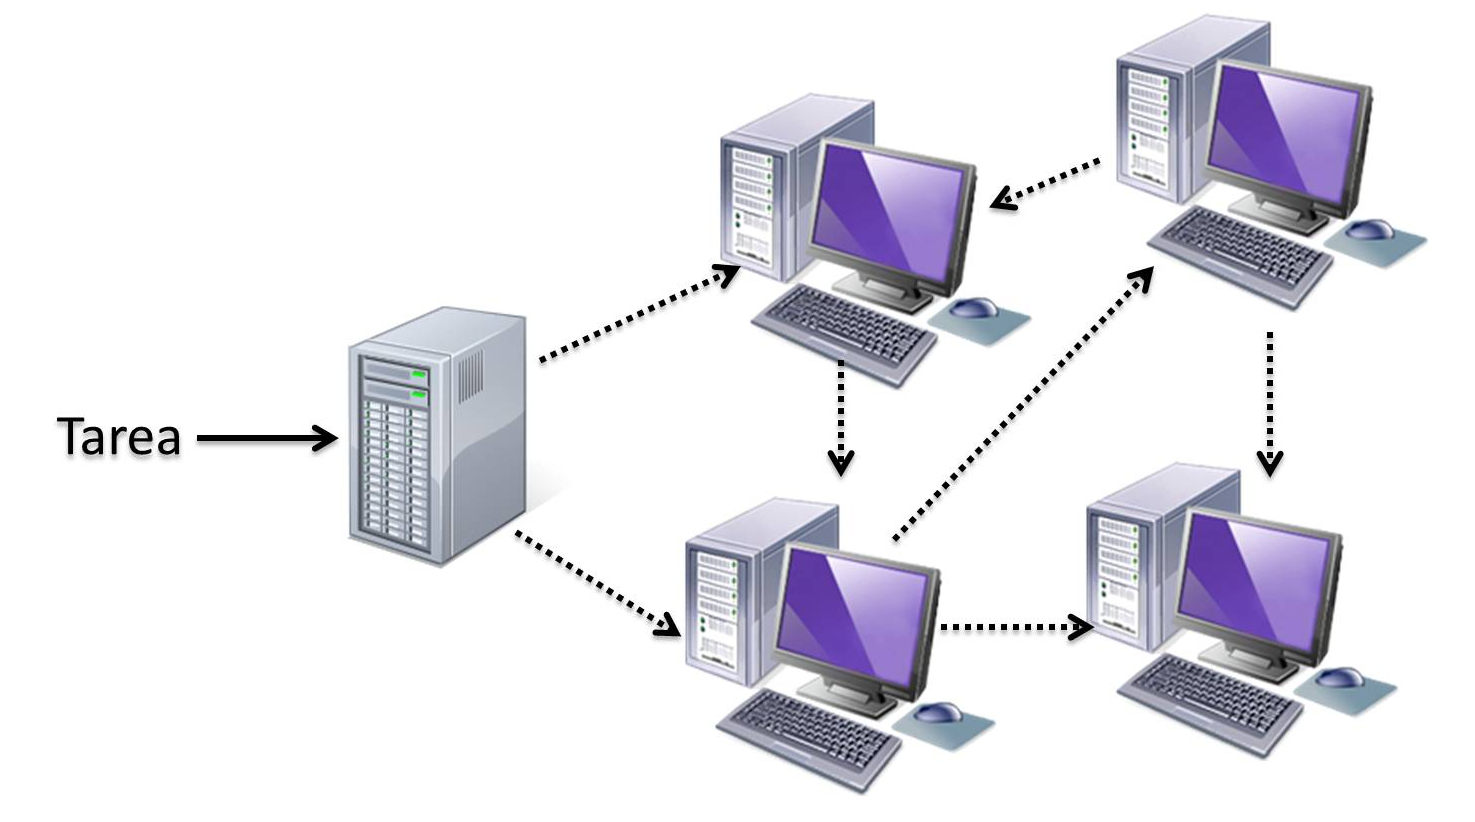
\includegraphics[scale=0.3]{graphics/computaciondistribuida}
\end{figure}

There are two main type of configurations on this system, the client-server, where there is a node which offers all the contents to other computers (the clients) which connect to the first one. This mode is used in the World Wide Web, but it has important problems, one produced when the server goes off, that the contents become unreachable and, other, when the server has a lot of connections stablished, because the performance is reduced.

The other mode is the peer-to-peer where all the computers of the network share the work between them and all the machines contribute with their memory and computation power. There is a variation of this configuration where there is a machine that control the network and the rest are the ones that make the work, this relation is called master-slave and it is the one which is going to be used in this project.

\subsection{Apache Spark}
\textit{Apache Spark} \cite{spark} is an open-source \gls{framework} that allows distributed data computation. It is developed in Scala \cite{scala}, but has support for Java, Python and R and it offers an \gls{API} to create distributed systems and deploy them to process data.

This \gls{API} is based in a data structure called Resilient Distributed Dataset (\gls{RDD}) where the data is stored, it has some qualities like its immutability, partitioning capacity and changes history that allows its parallel modification and to recover from failures. The framework uses the \gls{RAM} memory to store the data, being very quick the access to it. That makes \textit{Apache Spark} very good doing iterative jobs with the data.

\begin{figure}[htp!]
	\centering
	\caption{\textit{Apache Spark} components \cite{partsSpark}}
	\label{partSparkEng}
	\vspace{5pt}
	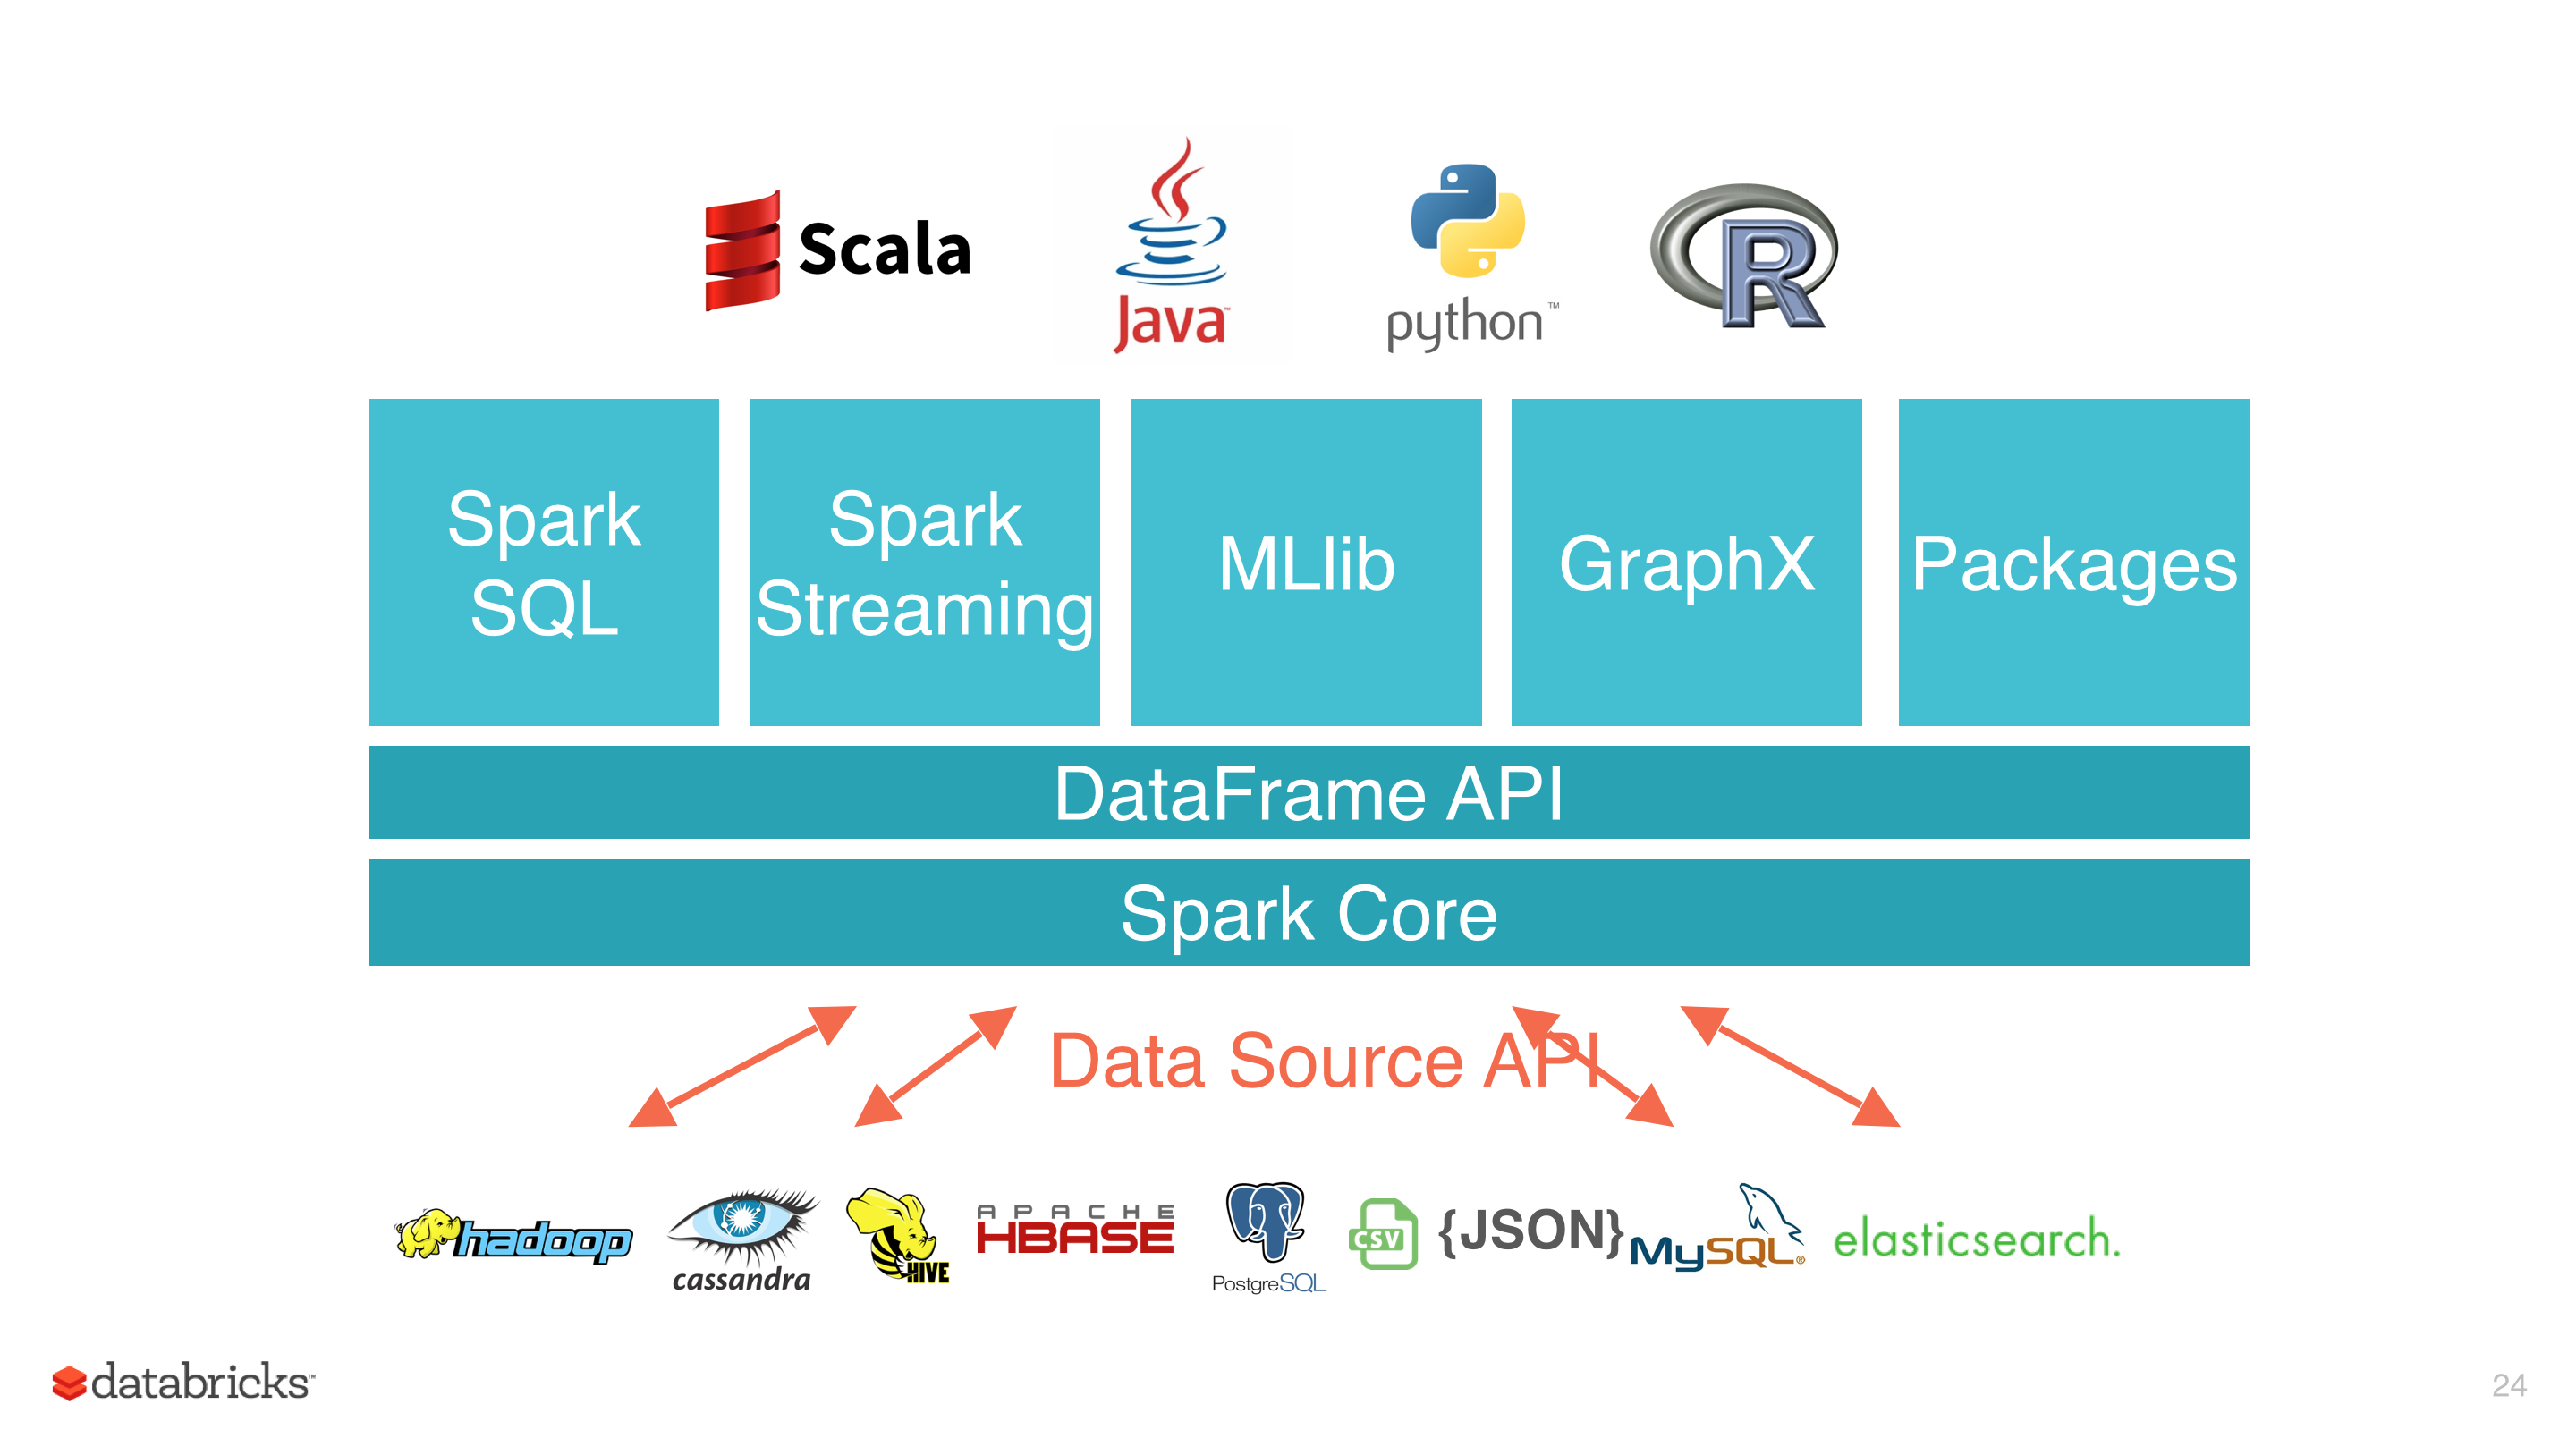
\includegraphics[scale=0.31]{graphics/partSpark}
\end{figure}

Other advantages of using \textit{Apache Spark} is its capacity to use most of file types to storage data and its integration with storage systems that facilitates the task of introducing data in the system. The framework also has some built-in libraries to do different task, these are:

\begin{itemize}
\item \textbf{Spark SQL:} That allows the use of structured and semi-structured data and the use of the SQL language to modify it.
\item \textbf{Spark Streaming:} That allows the analysis of real-time data with use of mini-batches generated with this data.
\item \textbf{MLib:} It is a machine learning library that allows the system to do different kind of analysis like clustering, classifications, regressions, etc.
\item \textbf{GraphX:} Allows parallel graph computation. Because of the immutability of the \gls{RDD}s it is not suitable for graphs that get updates.
\end{itemize}

\subsection{Apache Hadoop}
\textit{Apache Hadoop} \cite{hadoop} is another open-source \gls{framework} which enables the treatment of large datasets in a distributed way. Developed in Java it is used to manage distributed systems, being the fault-tolerance one of its most important qualities. 

It has four main modules, the Hadoop Common which supports the rest of them, the Hadoop Distributed File System (\gls{HDFS}) which is a distributed file system, Hadoop YARN which is a framework to manage the works of the nodes and Hadoop Mapreduce, based in YARN, it is used for parallel processing. In this project only the HDFS will be used, to replicate the data in the distributed configuration in the domestic cluster.

\gls{HDFS} is a distributed file system that gives to the system some important qualities in like replication of the data in the different nodes, fault-tolerance support and a way to save very large files. It uses a master-slave architecture.

\begin{figure}[htp!]
	\centering
	\caption{\gls{HDFS} architecture \cite{hadoop}}
	\label{hdfsarchitectureEng}
	\vspace{5pt}
	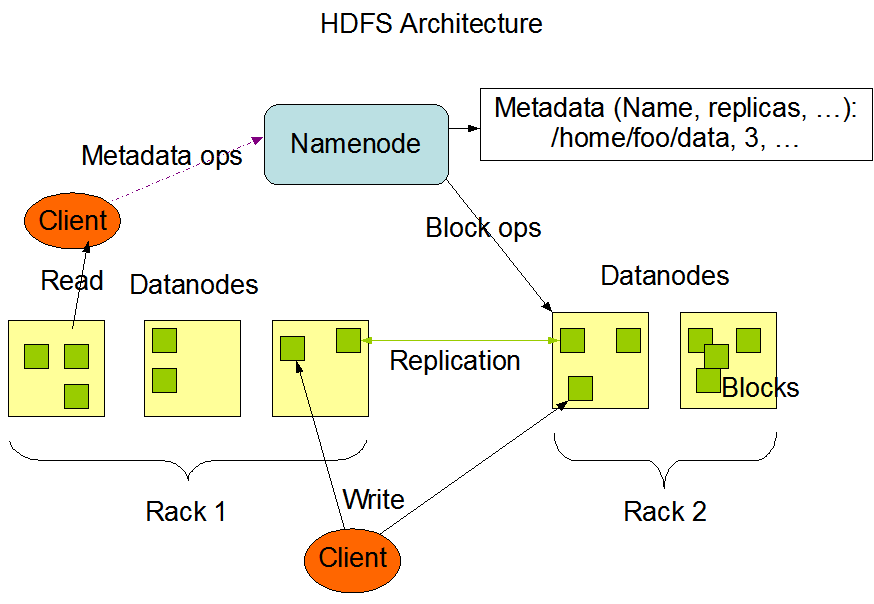
\includegraphics[scale=0.6]{graphics/hdfsarchitecture}
\end{figure}

\subsection{Apache Parquet}
\textit{Apache Parquet} \cite{parquet} is an open-source column-oriented file type of the Hadoop ecosystem, compatible with \textit{Apache Hadoop} and \textit{Spark}. It provides an efficient model of storage with an effective compression and codification system.

The columnar storage way saves the data table in columns rather than in rows being faster to access the data as it is not necessary to discard attributes to get the desired one. It is also better to store the data, especially in the case when the values repeat in some records.

In this project \textit{Snappy} \cite{snappyLib} will be used as the library to compress the data files, it fits very well because of the native support of the file type. This library doesn’t seek for the minimum file size, its best quality is its compression and extraction speed.

\begin{figure}[htp!]
	\centering
	\caption{Row and columnar storage models \cite{column}}
	\label{columnEng}
	\vspace{5pt}
	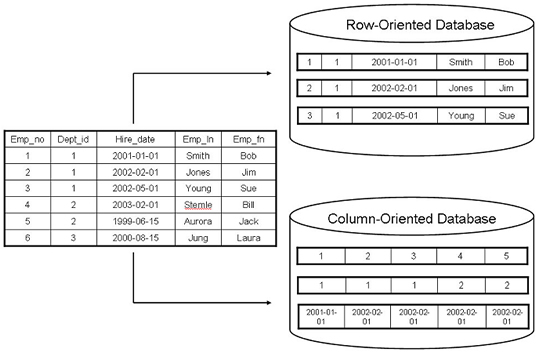
\includegraphics[scale=0.7]{graphics/column}
\end{figure}

\section{Design}
As it have been said, the goal of this project is the design and the implementation of a \textit{big data} architecture to process the traces of the taxi trips in New York city. Also, as another objective is to detect the limitations of the system in different environments, the implementation will be done in domestic and university ones that will make that the design suffers from some modifications depending of the execution environment.

The system will count with an only role, the administrator, that will be capable of doing all the task that the architecture will do, which are the load of the data, the process task of the data, the execution of the queries and the access to the results. For doing so, the system will count with three modules, described below:

\begin{itemize}
\item \textbf{Data loading and storage:} This module will take care of the data available in the system, will allow the user to upload the original traces of the challenge and, also, will be on charge of the data generated by the other modules.
\item \textbf{Data processing:} This module will be in charge of the data cleaning, eliminating the records with bad information, and of the data transformation, some attributes will change to adapt to the challenge rules.
\item \textbf{Query execution:} This module will provide the results to the problem through the execution of the queries exposed in the challenge.
\end{itemize}

These modules will interact among them and with the user to provide all the functionality of the system. 

On the other hand, as to the architecture of the system as it was said it will be implemented in two environments, the domestic and the university ones, and it also will allow two modes of execution, the pseudo-distributed where only one computer will be used and the distributed one, where there will be some machines.

As it was said, the pseudo-distributed system will count only with one computer. Thus, the jobs will be shared between the cores of the \gls{CPU}, one process will be the master of the rest and they will use de \gls{CPU} as needed. This kind of system have some advantages as they are easy to implement and to maintain but, on the other hand, it computational capacity is low compared with the distributed configuration.

\begin{figure}[htp!]
	\centering
	\caption{\textit{Apache Spark} distributed mode \cite{clusterfoto}}
	\label{fig:clusterSparkEN}
	\includegraphics[scale=0.6]{graphics/sparkCluster}
\end{figure} 

In the figure \ref{fig:clusterSparkEN} we can find the structure of a distributed system mounted with \textit{Apache Spark}, this will be the aspect of the multimode configuration on our system. As we can see, the master node will contain the \textit{SparkContext} job and will control the rest of the nodes.

This distributed system will count with two different implementations as two different environments will be used, these two designs will be:

\begin{itemize}
\item \textbf{Domestic cluster:} Will count with two laptops and one tower pc so the limit here will be the specs of the system, as the computers are low-tier ones. The main difference with the other cluster is the use of \gls{HDFS} to replicate the data between the computers, to eliminate big quantity data sending during the execution of the job. Figure \ref{domEN}
 
\item \textbf{University cluster:} In this case, the system count with a \gls{NFS} so the data is accessible by all the nodes of the architecture without doing any extra effort. This design is very similar to the pseudo-distributed one but using more machines. In this case, two, four, eight and sixteen nodes will be used. Figure \ref{uniEN}.
\end{itemize}

\begin{figure}[htp!]
\centering
\caption{Domestic cluster architecture}
\label{domEN}
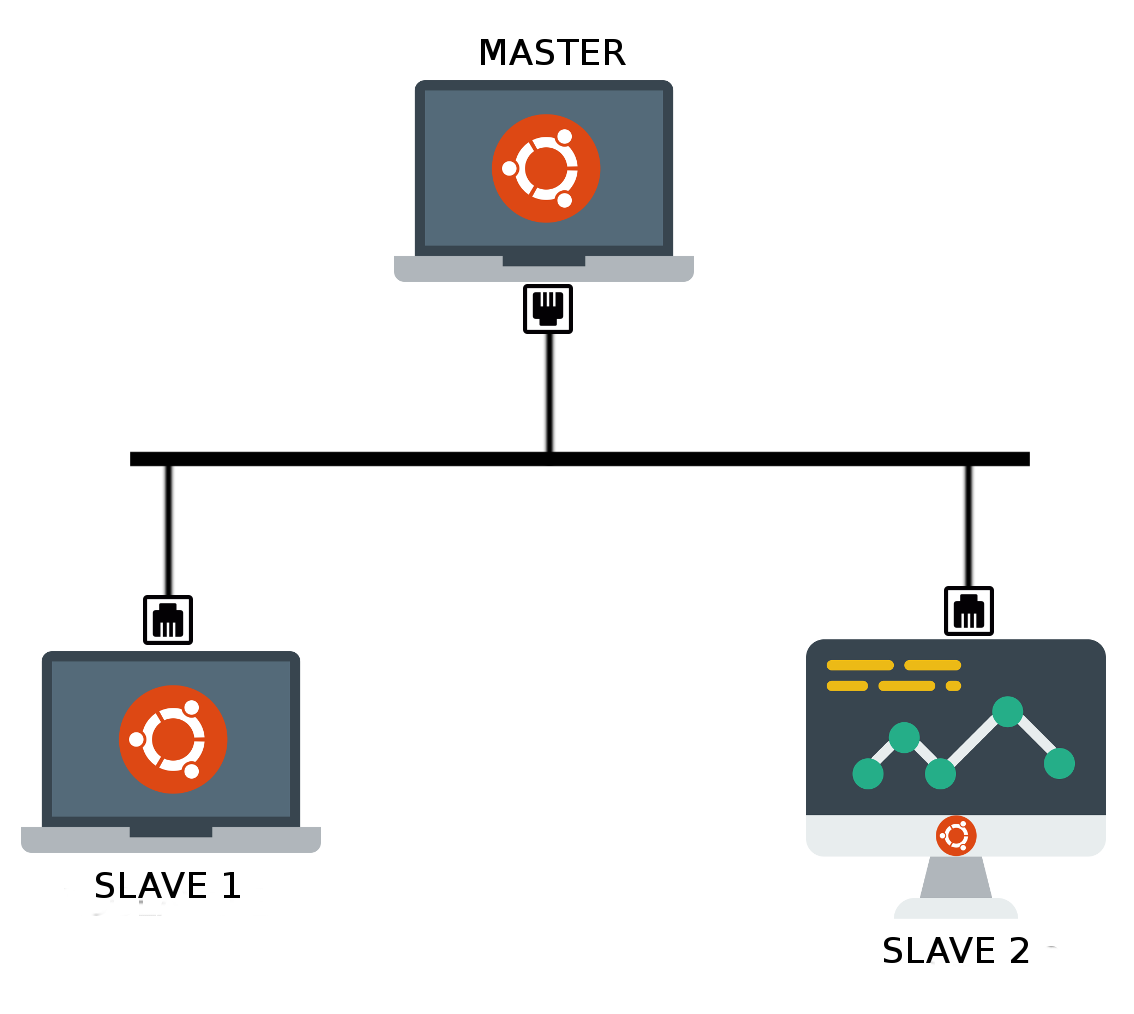
\includegraphics[scale=0.3]{graphics/DomENG}
\end{figure}

\begin{figure}[htp!]
\centering
\caption{University cluster architecture}
\label{uniEN}
\includegraphics[scale=0.25]{graphics/uniEN}
\end{figure}

\section{Implementation}
Three different configurations of the architecture will be implemented and tested in the two different environments commented. Although the core of the system will be the same for the three configurations, they will be based in \textit{Apache Spark}, the module of data processing and queries will be the same and they will be use \textit{Apache Parquet} as file type to save the data. These three configurations will be:

\begin{itemize}
\item Pseudo-distributed: This configuration will be tested in both environments and it has the easier configuration as it formed by one computer.
\item Domestic cluster: This configuration will be tested in the domestic environment with the configuration explained in the figure \ref{domEN}. It will use \textit{Apache Hadoop} as a data replication system is needed to make the data available in the slaves.
\item University cluster: This configuration will be tested in the university environment with the configuration explained in the figure \ref{uniEN}. It will use the \gls{NFS} available in the laboratory, so the data will be in each node without the necessity of a replication system.
\end{itemize}

To deploy the \textit{big data} system some steps will be needed before its implementation, this steps are the installation of Linux in the machines that will be used, the installation of Java, Scala, Python and \gls{SSH}, \textit{Apache Spark} and \textit{Apache Hadoop} (where is needed) in every machine utilised during this project. It is also required the configuration of the operating system, to stablish user groups and paths to avoid permission and execution problems, and the configuration of the technologies used to create the connections among the machines.

After this first steps, the implementation will require some steps to get a working system:

\begin{enumerate}
\item Obtaining the data.
\item Data loading.
\item Data analysis and processing.
\item Queries implementation.
\end{enumerate}

\subsection{Obtaining the data}
The file with all the taxi trips of Ney York city during 2013 is a 33 \gls{GB} \gls{CSV} file that can be downloaded from the webpage of the competition \cite{G
grandChallenge}. This file is called ``sorted\_data\_full.csv’’ and will be the base file for all the future work. It will be renamed to ```full.csv’’ and twelve more data files will be created from parts of its data, following the table \ref{ficherosCSV}.

\subsection{Data loading}
In this part, the data generated in the last step will be loaded in to the system to make it available for all the nodes of the system. In the case of the domestic cluster the data will be loaded through the command write in the code fragment \ref{cargaFicheroHDFS}

\subsection{Data analysis and processing}
In this step, after the analysis of the traces of the trip, the component in charge of cleaning and process the data will be developed. For the cleaning process, this module will remove from the data the records that have any kind of attribute with a wrong value, for example values with 0, and it also will check that the coordinates correspond with the city of New York, deleting the records that start or finish out of the city.

In the case of the processing task, the module will transform the data in different ways. First, for the correct implementation of the queries, the coordinates will be transformed to a grid with cells \ref{cuadricula}. Moreover, a new attribute with the day of the week of the trip will be added to facilitate filtering. Secondly, some attributes with no use in the queries will be deleted saving disk space.

\subsection{Implementation of the queries}
The challenge asked for two queries over the data given, but for this project, the final number of queries implemented is four because a modification over the original queries have been made to take seasonality of the data in mind, increasing the computational needs. 

These modifications have been made to test the capacity of the system when a lot of operations are needed to obtain the results, as an influence factor have been added to calculate the influence of the trips depending of the date. In summary, these modifications take in consideration all the trips of the data file and make float operations to calculate the influence in the final results, needing more resources to be executed than the originals, which limit the data to a time window.

The queries implemented had been:

\begin{itemize}
\item \textbf{Frequent routes:} This query return the top 10 most frequent routes during the last 30 minutes. 
\item \textbf{Frequent routes with seasonality:} This query return the top 10 most frequent routes taking in mind a time window of thirty minutes and the day of the week. This query search in all the trips that adjust to these attributes and calculate its influence depending of the difference of dates.
\item \textbf{Profitable areas:} This query return the top ten areas that are currently most profitable for taxi drivers. The profitability of a zone its calculated with the price paid for the trips started in the zona during the last 15 minutes divided for the number of free taxis in the zone.
\item \textbf{Profitable areas with seasonality:} This query return the top ten areas that are currently most profitable for taxi drivers. As the other query with seasonality it takes in consideration all the trips made during the day of the week and the time window stablished.
\end{itemize}

\section{Results}
In this section, we will analyse the results obtained after making the test to the different configurations of the system and environments. This test will focus in two factors, first, the number of nodes of the system, comparing the results of the different numbers. Secondly, the size of the dataset, comparing the results using different sizes of the file with the trips.

\subsection{Test environments}
As it has been said, there will be two main modes of execution in the system, the pseudo-distributed and the distributed, and, also, there are two environments, the domestic and the university one.

The pseudo-distributed mode will we tried in every environment and will be used as guide to comparing the time with the distributed time. In the case of the distributed mode, there are different implementations for each environment. The university cluster will count with more test as the number of nodes will change to compare the scalability of the architecture.

The pseudo-distributed configuration will count with the computer of the table \ref{maestroDomestico} whereas in the university will be the computer of the table \ref{equipoUniversitario}. In the case of the distributed configuration, in the domestic cluster the master will be the computer of the table \ref{maestroDomestico} and the slaves will be the ones on the tables \ref{esclavo1} and \ref{esclavo2}. In the university lab all the machines are the same, the one of the table \ref{equipoUniversitario}.

\subsection{Data files}
As it was commented during the implementation phase, the system will use \textit{Apache Parquet} to save the clean and processed data. The decision was taken because this file type had better read speeds and because of its compression system, that allow us to compress the 33 \gls{GB} file to another of less than 5 GB.

The speed and size comparison could be seen in the tables \ref{velocidadCSVEN} and \ref{velocidadParquetEN}.

\begin{table}[htp!]
	\centering
	\caption{Files and read test for \gls{CSV}}
	\label{velocidadCSVEN}
	\begin{tabular}{|l|l|l|l|l|}
		\hline
		\multicolumn{5}{|c|}{\textbf{CSV}}                                                                               \\ \hline
		\textbf{Filename} & \textbf{Records} & \textbf{Size (GB)} & \textbf{Time (seg)} & \textbf{Records/seg} \\ \hline
		mil.csv         & 173185             & 0,032519531     & 0,99720043                 & 173671                     \\ \hline
		quinientos.csv  & 346370             & 0,065039063     & 1,959946904                & 176724                     \\ \hline
		cinquenta.csv   & 3463702            & 0,649707031     & 15,24788392                & 227159                     \\ \hline
		1decimo.csv     & 17318509           & 3,3             & 494,5507809                & 35018                      \\ \hline
		2decimo.csv     & 34637018           & 6,7             & 389,0821234                & 89022                      \\ \hline
		3decimo.csv     & 51955527           & 10              & 291,1400167                & 178455                     \\ \hline
		4decimo.csv     & 69274036           & 13,3            & 182,5482055                & 379483                     \\ \hline
		half.csv        & 86592546           & 16,6            & 86,86696803                & 996840                     \\ \hline
		6decimo.csv     & 103911055          & 20              & 585,2277942                & 177556                     \\ \hline
		7decimo.csv     & 121229563          & 23,3            & 703,9244393                & 172219                     \\ \hline
		8decimo.csv     & 138548072          & 26,6            & 827,5500103                & 167419                     \\ \hline
		9decimo.csv     & 155866581          & 30              & 952,5683697                & 163627                     \\ \hline
		full.csv        & 173185091          & 33,3            & 978,0770412                & 177066                     \\ \hline
		&                    &                      & \textbf{Tiempo total (seg)} & \textbf{Media reg/seg}     \\ \hline
		&                    &                 & 5509,740781                & 239558,3846                \\ \hline
	\end{tabular}
\end{table}

\begin{table}[htp!]
	\centering
	\caption{Files and read test for \textit{Parquet}}
	\label{velocidadParquetEN}
	\begin{tabular}{|l|l|l|l|l|}
		\hline
		\multicolumn{5}{|c|}{\textbf{PARQUET + SNAPPY}}                                                                          \\ \hline
		\textbf{Filename} & \textbf{Records} & \textbf{Size (GB)} & \textbf{Time (seg)} & \textbf{Records/seg} \\ \hline
		mil.parquet        & 166570             & 0,0078125            & 0,088930148                 & 1873043                    \\ \hline
		quinientos.parquet & 333971             & 0,012304688          & 0,10375922                  & 3218711                    \\ \hline
		cinquenta.parquet  & 3341159            & 0,089160156          & 0,13233389                  & 25247946                   \\ \hline
		1decimo.parquet    & 16716605           & 0,44140625           & 0,533758281                 & 31318680                   \\ \hline
		2decimo.parquet    & 33428358           & 0,883789063          & 1,172321222                 & 28514674                   \\ \hline
		3decimo.parquet    & 50192489           & 1,32                 & 1,802668324                 & 27843440                   \\ \hline
		4decimo.parquet    & 66932537           & 1,76                 & 2,563482635                 & 26110002                   \\ \hline
		half.parquet       & 83216713           & 2,2                  & 3,21071474                  & 25918438                   \\ \hline
		6decimo.parquet    & 100048869          & 2,65                 & 3,437491023                 & 29105201                   \\ \hline
		7decimo.parquet    & 116946068          & 3,11                 & 6,598058132                 & 17724316                   \\ \hline
		8decimo.parquet    & 133836035          & 3,56                 & 10,72142728                 & 12483042                   \\ \hline
		9decimo.parquet    & 150630563          & 4,01                 & 8,413226073                 & 17904019                   \\ \hline
		full.parquet       & 167361464          & 4,46                 & 19,46584598                 & 8597697                    \\ \hline
		                   &                    &                      & \textbf{Tiempo total (seg)} & \textbf{Media reg/seg}     \\ \hline
						   &                    &                      & 58,24401784                 & 19681477,62                \\ \hline
	\end{tabular}
\end{table}

\subsection{Architecture performance}
In this chapter, the results obtained with the different configurations of the system will be analysed, first, the ones obtained in the domestic environment and then, the ones obtained in the university environment, which represents better a real situation as all the machines has the same specs.

The test made measure three aspects of the systems, related among them, but necessary to understand the performance. This three aspects are:

\begin{itemize}
	\item \textbf{Time:} Elapsed time to complete the task in seconds.
	\item \textbf{Speed:} Quantity of records processed per second during the realisation of the task $speed = \dfrac{nº \; of \; records}{execution \; time}$
	\item \textbf{Efficiency:} Speed divide by the system cores. \cite{eficiencia}. $efficiency = \dfrac{speed}{nº \; of \; cores}$
\end{itemize}

The obtained results could be seen in the following graphs. If we look to the results, the first thing that one notice is that the distributed configurations are less time efficient than the pseudo-distributed one until the size of the file is big enough. This is one of the premises of \textit{big data}. This problem is bigger in the queries that don’t require a lot of computation, because the threshold is higher in these cases. This is caused because of the time lost in the distribution of the task between the nodes.

Other visible aspect, especially in the university cluster where the configurations follow a linear incrementation of the resources, is that the time required for finishing the task is inversely proportional to the increase in specs of the cluster. In other words, if the specs of one configuration is the double to the specs of other, the execution time will be nearly the half of the time.

This aspect, although it is true for configurations with low number of nodes, for example, going from two to four nodes, in the case of big numbers it is not always true, for example, from eight to sixteen nodes. This is caused because at that levels the specs increase provided do not worth the latency time between the nodes.

Thus, a balance between the number of nodes and the latency between them should be seek for the most efficient system. Another conclusion that we can extract from the results obtained is that in this architecture the number of cores in the system were more determining than the \gls{RAM}. This was caused because of the compression of the data, as we have the data compressed the \gls{CPU} were more necessary to get access the data. 

Nevertheless, it could be seen how having limited memory affects to the system, loosing efficiency as disk accesses were necessary, which is a slower operation compared with the access to \gls{RAM} memory.


\subsubsection{Domestic cluster}
\begin{figure}[htp!]
	\centering
	\caption{Data processing time domestic cluster}
	\label{tpd}
	\vspace{5pt}
	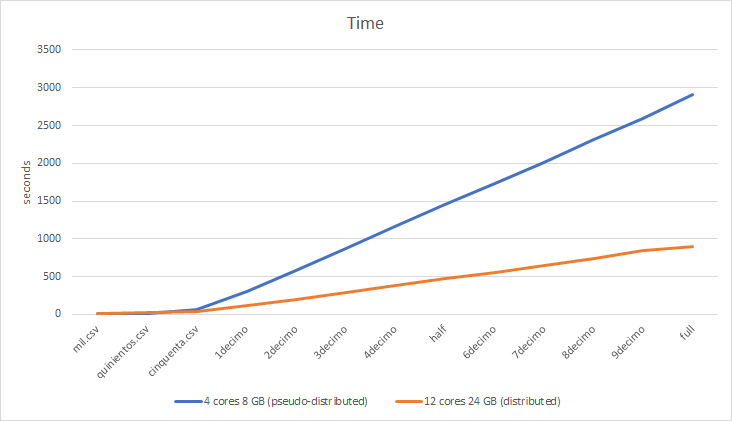
\includegraphics[scale=0.8]{geng/tpd}
\end{figure}
\begin{figure}[htp!]
	\centering
	\caption{Data processing speed domestic cluster}
	\label{spd}
	\vspace{5pt}
	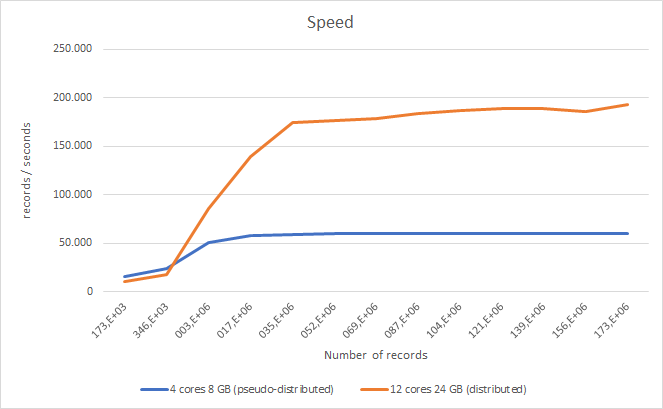
\includegraphics[scale=0.85]{geng/spd}
\end{figure}
\begin{figure}[htp!]
	\centering
	\caption{Data processing efficiency domestic cluster}
	\label{epd}
	\vspace{5pt}
	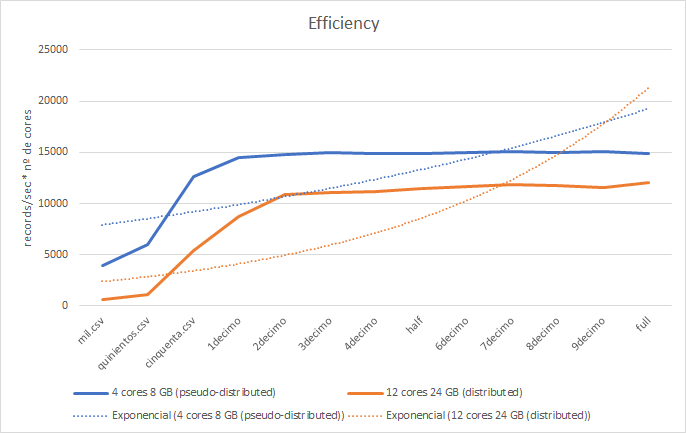
\includegraphics[scale=0.85]{geng/epd}
\end{figure}

\begin{figure}[htp!]
	\centering
	\caption{Frequent routes time domestic cluster}
	\label{tfd}
	\vspace{5pt}
	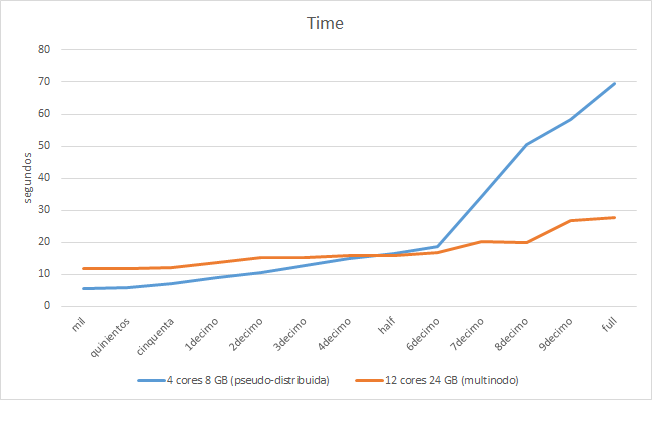
\includegraphics[scale=0.8]{geng/tfd}
\end{figure}
\begin{figure}[htp!]
	\centering
	\caption{Frequent routes speed domestic cluster}
	\label{sfd}
	\vspace{5pt}
	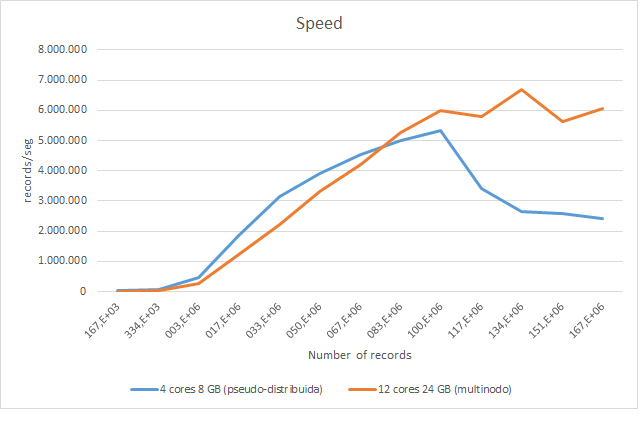
\includegraphics[scale=0.85]{geng/sfd}
\end{figure}
\begin{figure}[htp!]
	\centering
	\caption{Frequent routes efficiency domestic cluster}
	\label{efd}
	\vspace{5pt}
	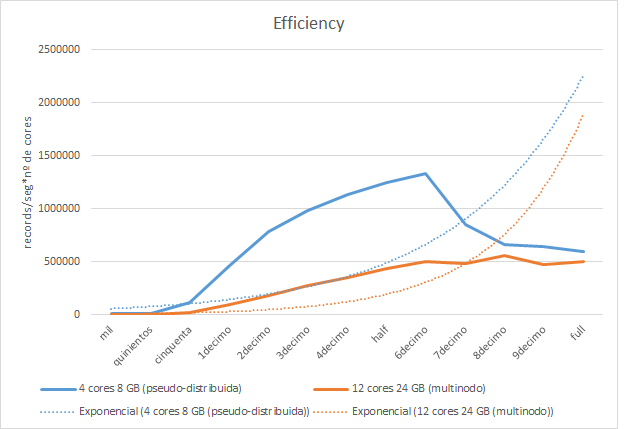
\includegraphics[scale=0.85]{geng/efd}
\end{figure}

\begin{figure}[htp!]
	\centering
	\caption{Frequent routes with seasonality time domestic cluster}
	\label{tfdd}
	\vspace{5pt}
	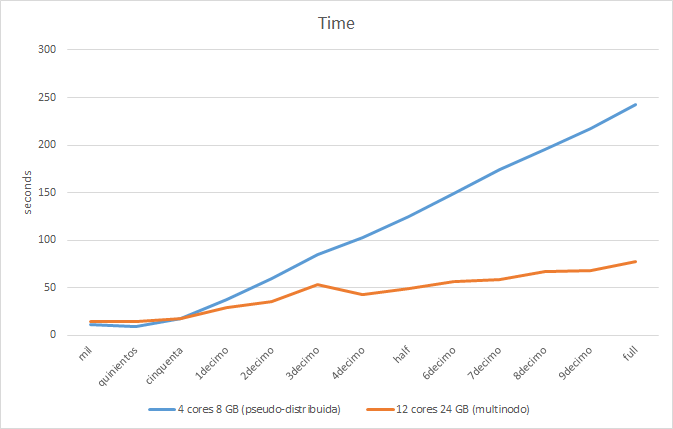
\includegraphics[scale=0.8]{geng/tfdd}
\end{figure}
\begin{figure}[htp!]
	\centering
	\caption{Frequent routes with seasonality speed domestic cluster}
	\label{sfdd}
	\vspace{5pt}
	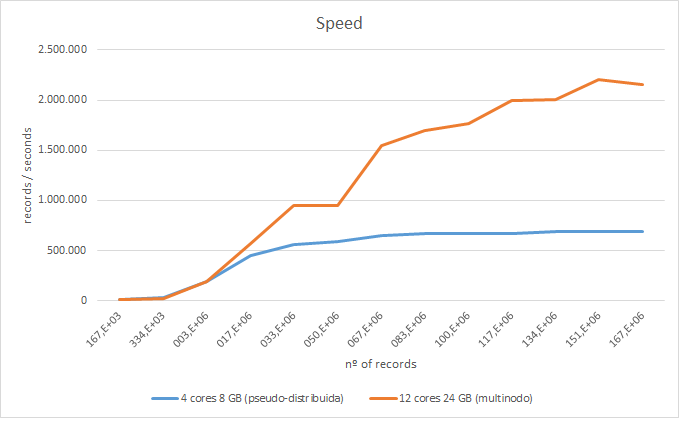
\includegraphics[scale=0.85]{geng/sfdd}
\end{figure}
\begin{figure}[htp!]
	\centering
	\caption{Frequent routes with seasonality domestic cluster}
	\label{efdd}
	\vspace{5pt}
	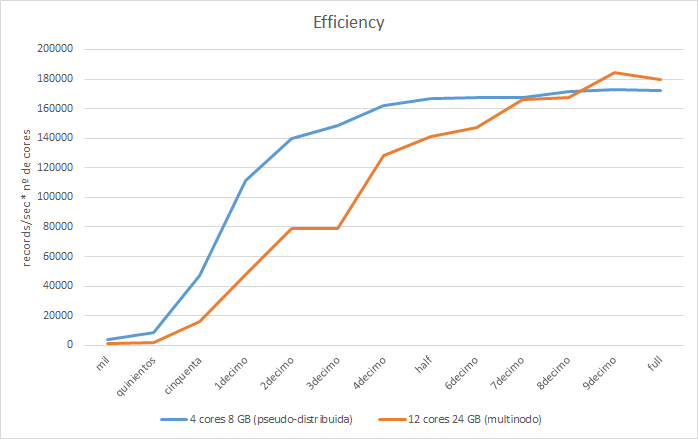
\includegraphics[scale=0.85]{geng/efdd}
\end{figure}

\begin{figure}[htp!]
	\centering
	\caption{Profitable zones time domestic cluster}
	\label{tprd}
	\vspace{5pt}
	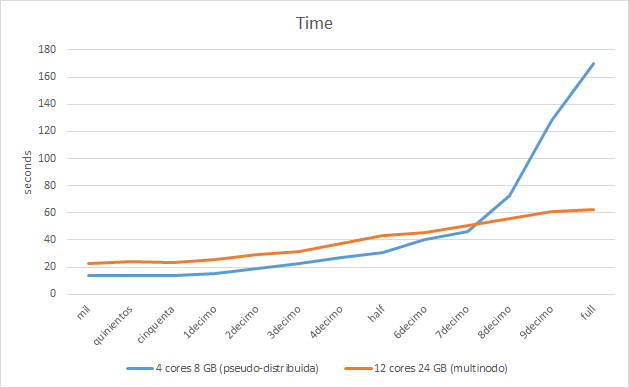
\includegraphics[scale=0.8]{geng/tprd}
\end{figure}
\begin{figure}[htp!]
	\centering
	\caption{Profitable zones speed domestic cluster}
	\label{sprd}
	\vspace{5pt}
	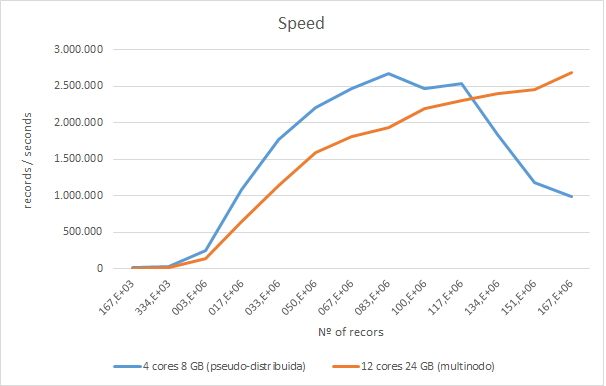
\includegraphics[scale=0.85]{geng/sprd}
\end{figure}
\begin{figure}[htp!]
	\centering
	\caption{Profitable zones efficiency domestic cluster}
	\label{eprd}
	\vspace{5pt}
	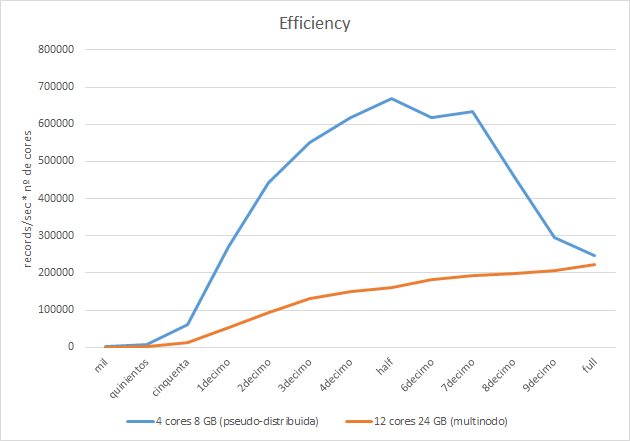
\includegraphics[scale=0.85]{geng/eprd}
\end{figure}

\begin{figure}[htp!]
	\centering
	\caption{Profitable zones with seasonality time domestic cluster}
	\label{tpdd}
	\vspace{5pt}
	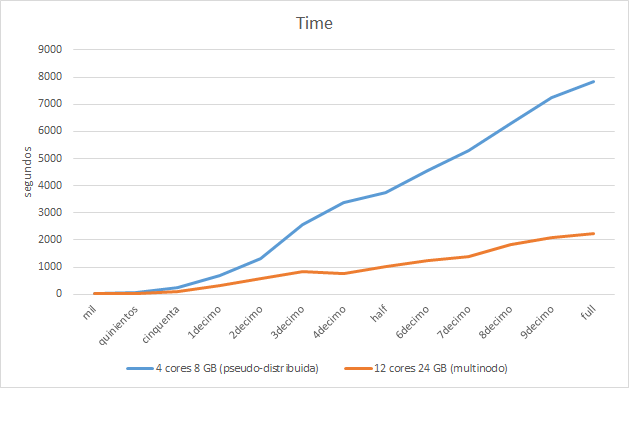
\includegraphics[scale=0.8]{geng/tpdd}
\end{figure}
\begin{figure}[htp!]
	\centering
	\caption{Profitable zones with seasonality speed domestic cluster}
	\label{spdd}
	\vspace{5pt}
	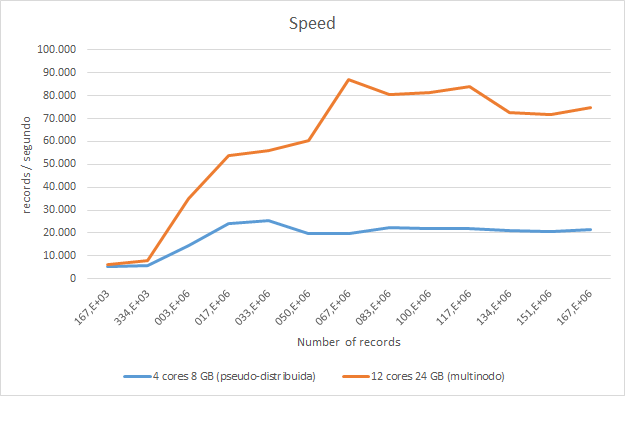
\includegraphics[scale=0.85]{geng/spdd}
\end{figure}
\begin{figure}[htp!]
	\centering
	\caption{Profitable zones with seasonality efficiency domestic cluster}
	\label{epdd}
	\vspace{5pt}
	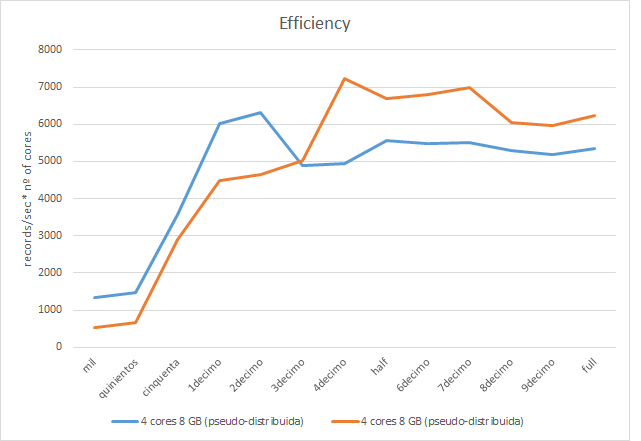
\includegraphics[scale=0.85]{geng/epdd}
\end{figure}

\subsubsection{University cluster}
\begin{figure}[htp!]
	\centering
	\caption{Data processing time university cluster}
	\label{tpu}
	\vspace{5pt}
	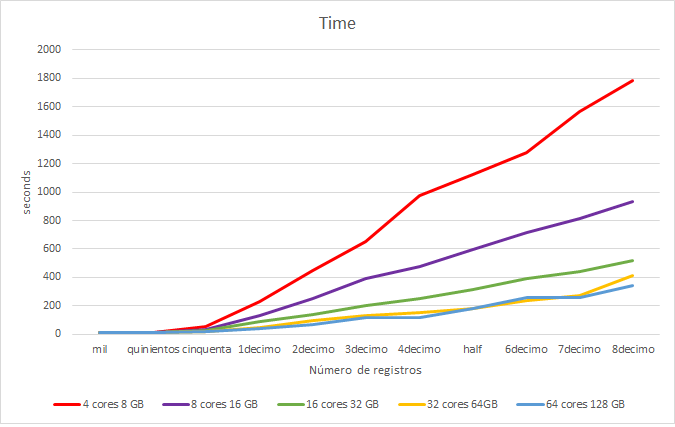
\includegraphics[scale=0.8]{geng/tpu}
\end{figure}
\begin{figure}[htp!]
	\centering
	\caption{Data processing speed university cluster}
	\label{spu}
	\vspace{5pt}
	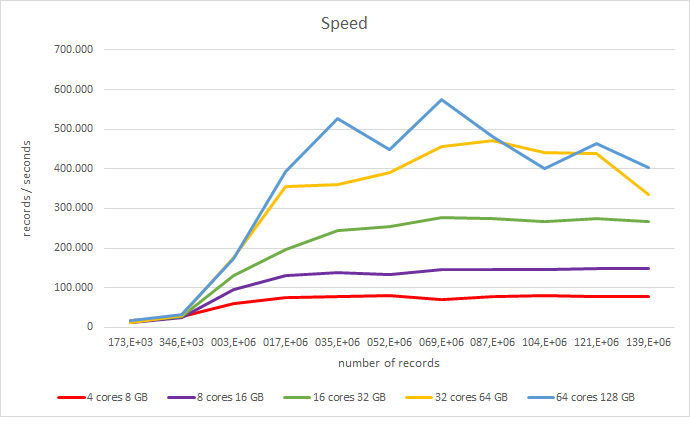
\includegraphics[scale=0.85]{geng/spu}
\end{figure}
\begin{figure}[htp!]
	\centering
	\caption{Data processing efficiency university cluster}
	\label{epu}
	\vspace{5pt}
	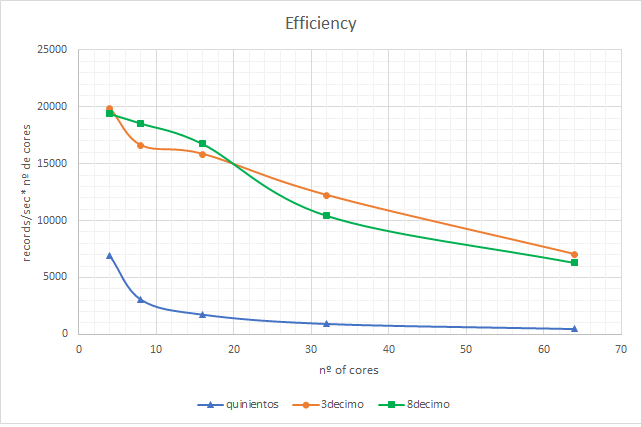
\includegraphics[scale=0.85]{geng/epu}
\end{figure}

\begin{figure}[htp!]
	\centering
	\caption{Frequent routes time university cluster}
	\label{tfu}
	\vspace{5pt}
	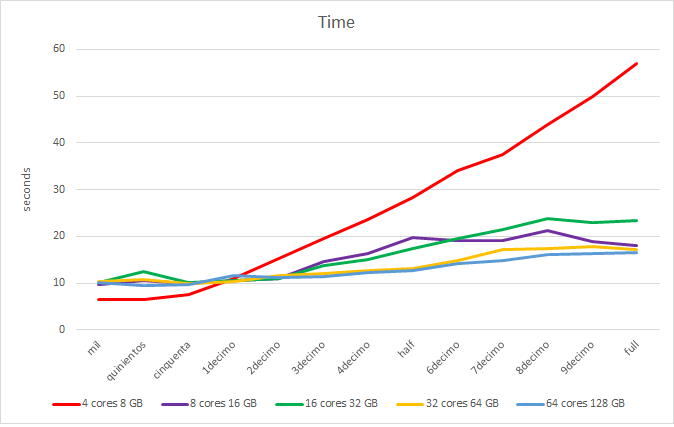
\includegraphics[scale=0.8]{geng/tfu}
\end{figure}
\begin{figure}[htp!]
	\centering
	\caption{Frequent routes speed university cluster}
	\label{sfu}
	\vspace{5pt}
	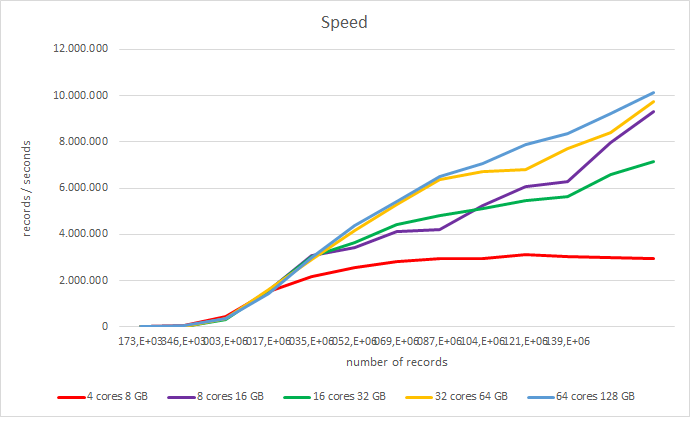
\includegraphics[scale=0.85]{geng/sfu}
\end{figure}
\begin{figure}[htp!]
	\centering
	\caption{Frequent routes efficiency university cluster}
	\label{efu}
	\vspace{5pt}
	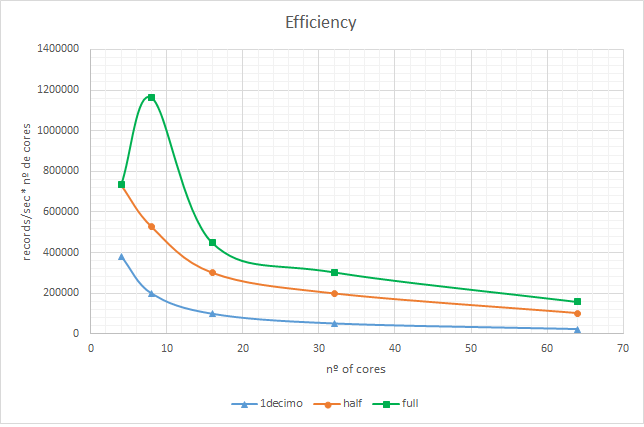
\includegraphics[scale=0.85]{geng/efu}
\end{figure}

\begin{figure}[htp!]
	\centering
	\caption{Frequent routes with seasonality time university cluster}
	\label{tfdu}
	\vspace{5pt}
	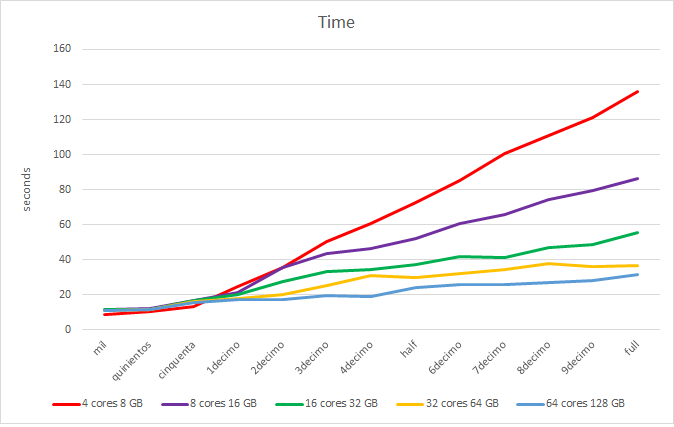
\includegraphics[scale=0.8]{geng/tfdu}
\end{figure}
\begin{figure}[htp!]
	\centering
	\caption{Frequent routes with seasonality speed university cluster}
	\label{sfdu}
	\vspace{5pt}
	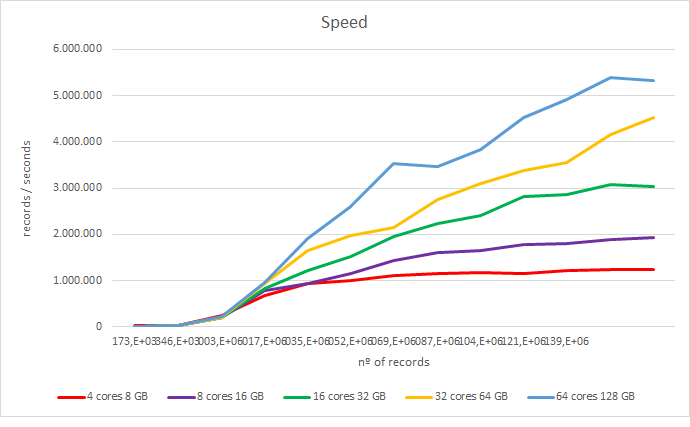
\includegraphics[scale=0.85]{geng/sfdu}
\end{figure}
\begin{figure}[htp!]
	\centering
	\caption{Frequent routes with seasonality university cluster}
	\label{efdu}
	\vspace{5pt}
	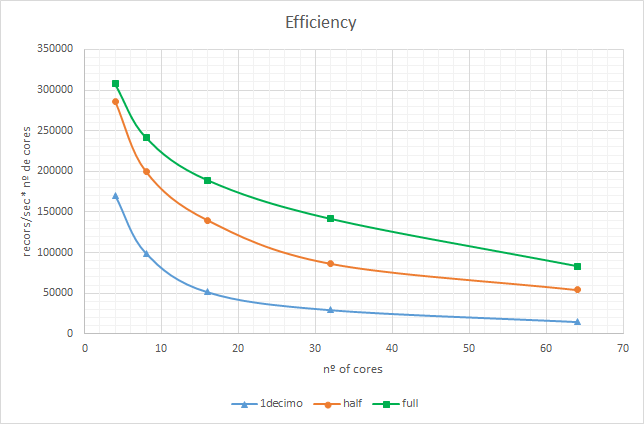
\includegraphics[scale=0.85]{geng/efdu}
\end{figure}

\begin{figure}[htp!]
	\centering
	\caption{Profitable zones time university cluster}
	\label{tpru}
	\vspace{5pt}
	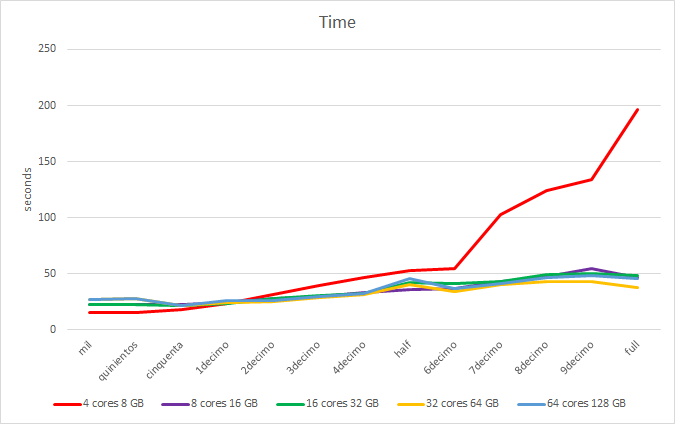
\includegraphics[scale=0.8]{geng/tpru}
\end{figure}
\begin{figure}[htp!]
	\centering
	\caption{Profitable zones speed university cluster}
	\label{spru}
	\vspace{5pt}
	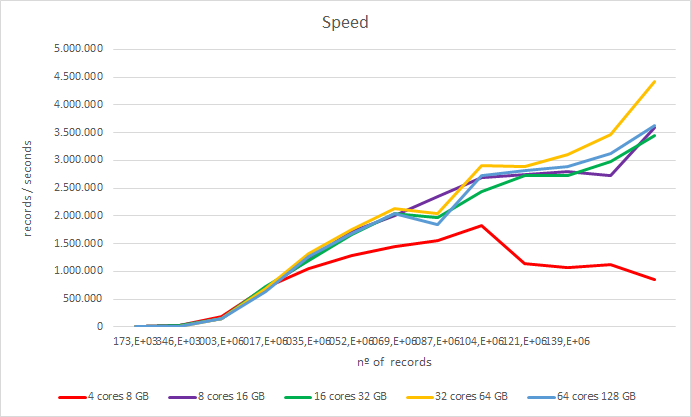
\includegraphics[scale=0.85]{geng/spru}
\end{figure}
\begin{figure}[htp!]
	\centering
	\caption{Profitable zones efficiency university cluster}
	\label{epru}
	\vspace{5pt}
	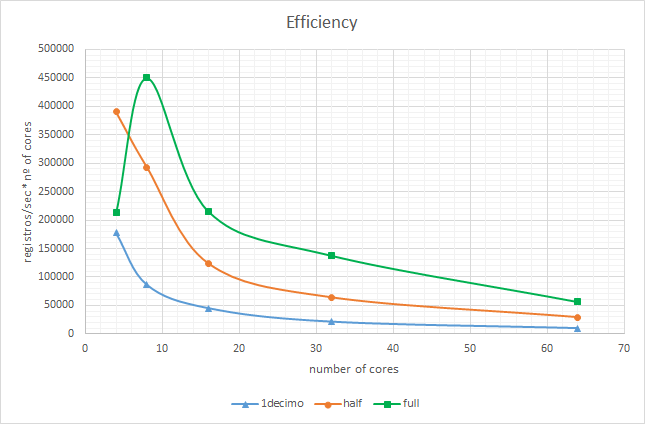
\includegraphics[scale=0.85]{geng/epru}
\end{figure}

\begin{figure}[htp!]
	\centering
	\caption{Profitable zones with seasonality time university cluster}
	\label{tpdu}
	\vspace{5pt}
	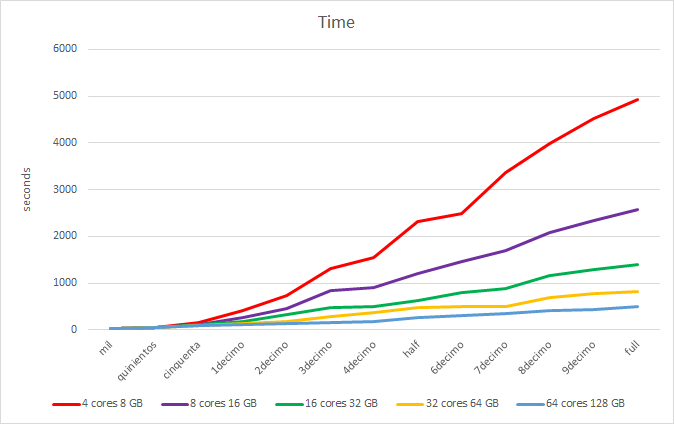
\includegraphics[scale=0.8]{geng/tpdu}
\end{figure}
\begin{figure}[htp!]
	\centering
	\caption{Profitable zones with seasonality speed university cluster}
	\label{spdu}
	\vspace{5pt}
	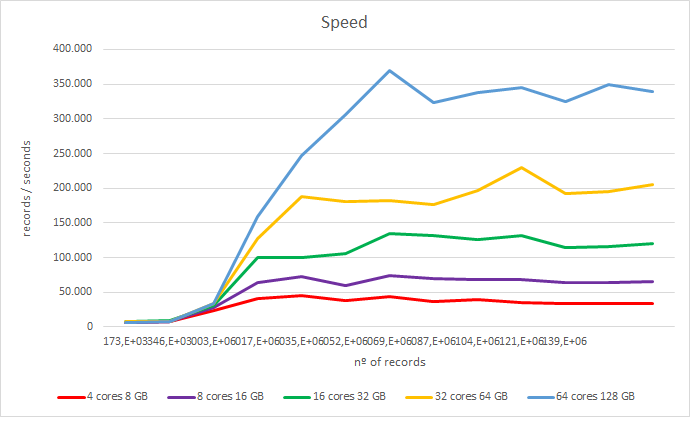
\includegraphics[scale=0.85]{geng/spdu}
\end{figure}
\begin{figure}[htp!]
	\centering
	\caption{Profitable zones with seasonality efficiency university cluster}
	\label{epdu}
	\vspace{5pt}
	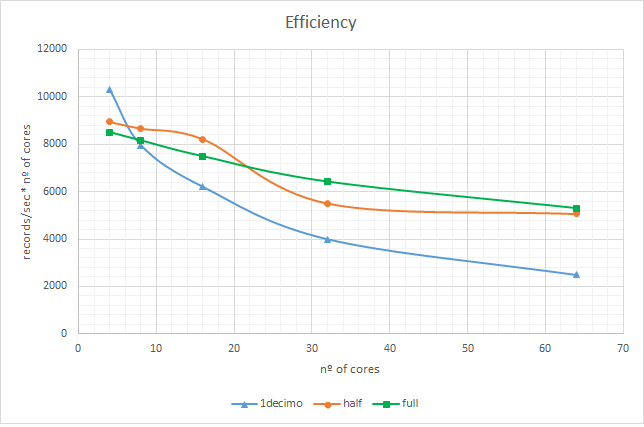
\includegraphics[scale=0.85]{geng/epdu}
\end{figure}